\section{Concentration Dependent Boundary Condition}
\label{ch:results-analysis}
\subsection{Time evolution}

In this chapter we discus the results obtained by the dynamic algorithm. We study different parameter regimes and the behaviour of the electric potential and electric field.

We are interested in studying the time evolution of the system from initial conditions. Figure \ref{fig:ef1} shows the time evolution of the system for a time window of $t = 4.48 ns$




\begin{figure}[htbp]
\centering
\textbf{Electric Field In The Diffusion Problem With Nernst Interaction.}\par\medskip
\begin{subfigure}{.5\linewidth}
\centering
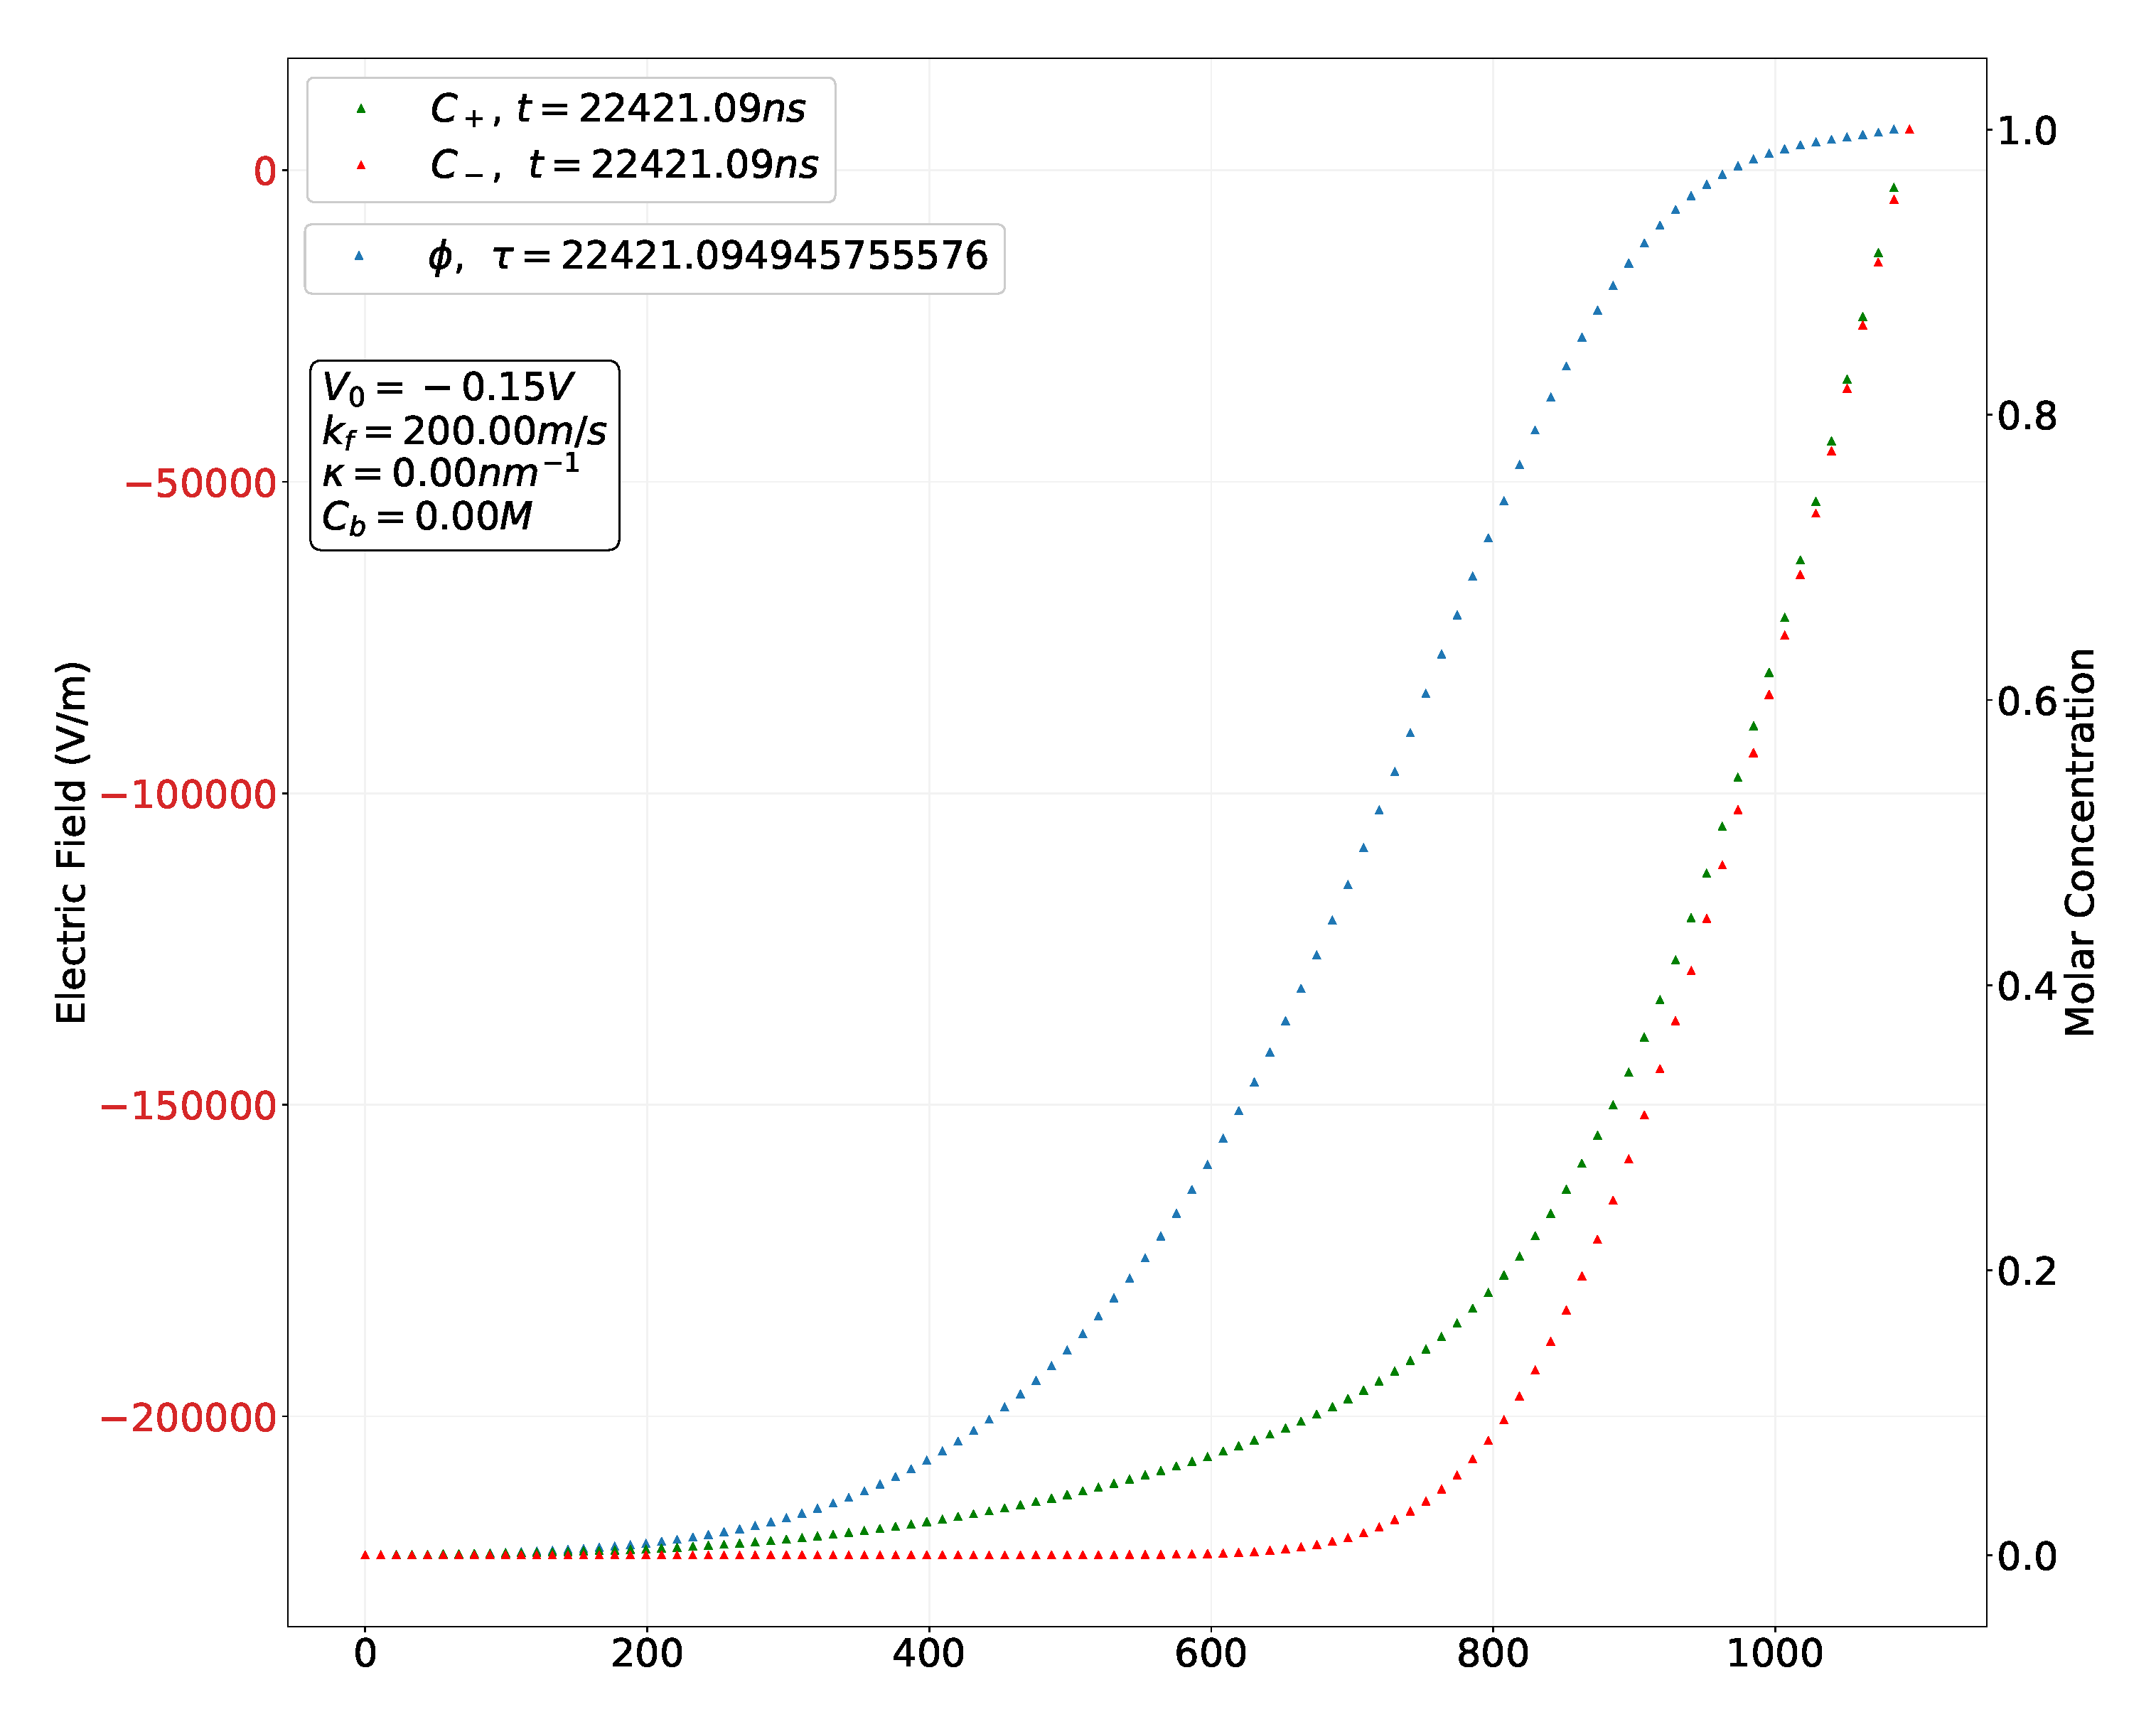
\includegraphics[width=\textwidth]{langmuir-diffusion-nernstE0.eps}
\caption{}
\label{fig:time-evol1_1}
\end{subfigure}%
\begin{subfigure}{.5\linewidth}
\centering
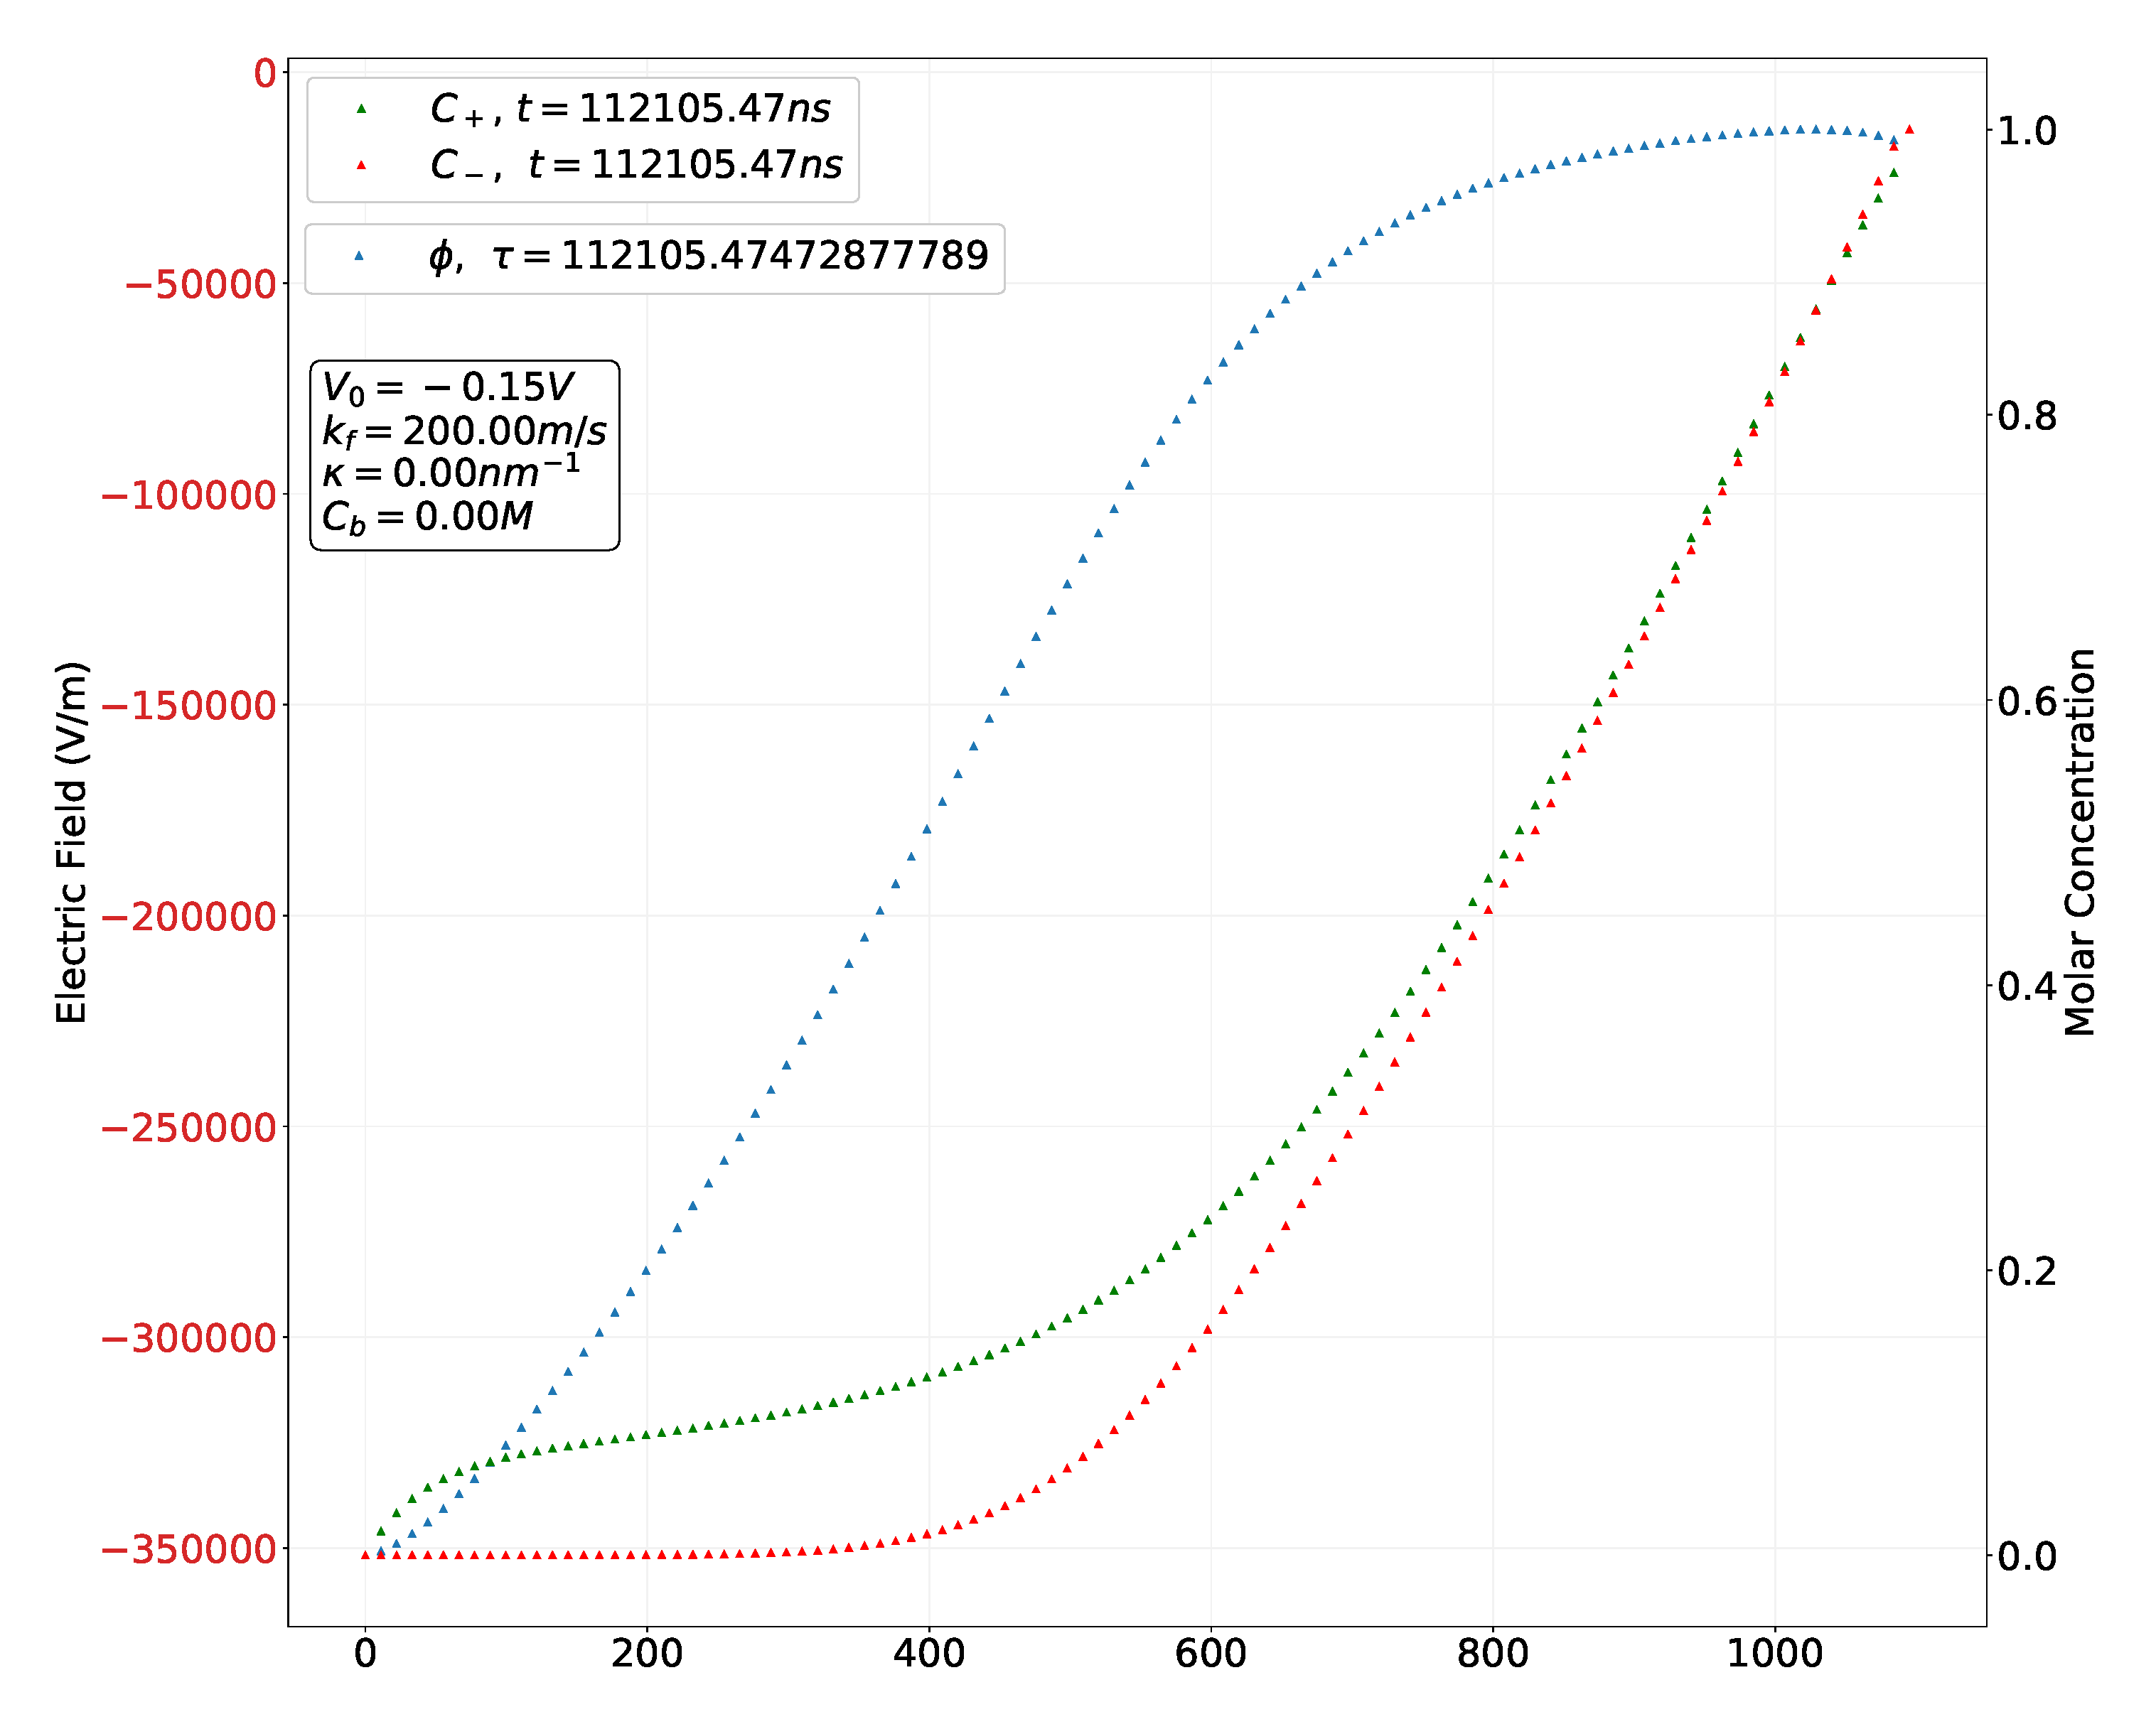
\includegraphics[width =\textwidth]{langmuir-diffusion-nernstE1.eps}
\caption{}
\label{fig:time-evol1_2}
\end{subfigure}\\[1ex]
\begin{subfigure}{\linewidth}
\centering
\includegraphics[width =0.5\textwidth]{langmuir-diffusion-nernstE2.eps}
\caption{}
\label{fig:time-evol1_3}
\end{subfigure}
\caption{Electric field and concentration of $Cu^{+2}$ (green dots) and $SO_4^{-2}$ (blue dots) at (a) $t = 0.448 ns$, (b) $t = 2.24 ns$ and (c) $t = 4.44 ns$. Steady state is reached in times greater than $t = 4.44 ns$.}
\end{figure}

\begin{figure}[htbp]
\centering
\textbf{Electric Potential In The Diffusion Problem With Nernst Interaction.}\par\medskip
\begin{subfigure}{.5\linewidth}
\centering
\includegraphics[width=\textwidth]{langmuir-diffusion-nernstphi0.eps}
\caption{}
\label{fig:time-evol2_1}
\end{subfigure}%
\begin{subfigure}{.5\linewidth}
\centering
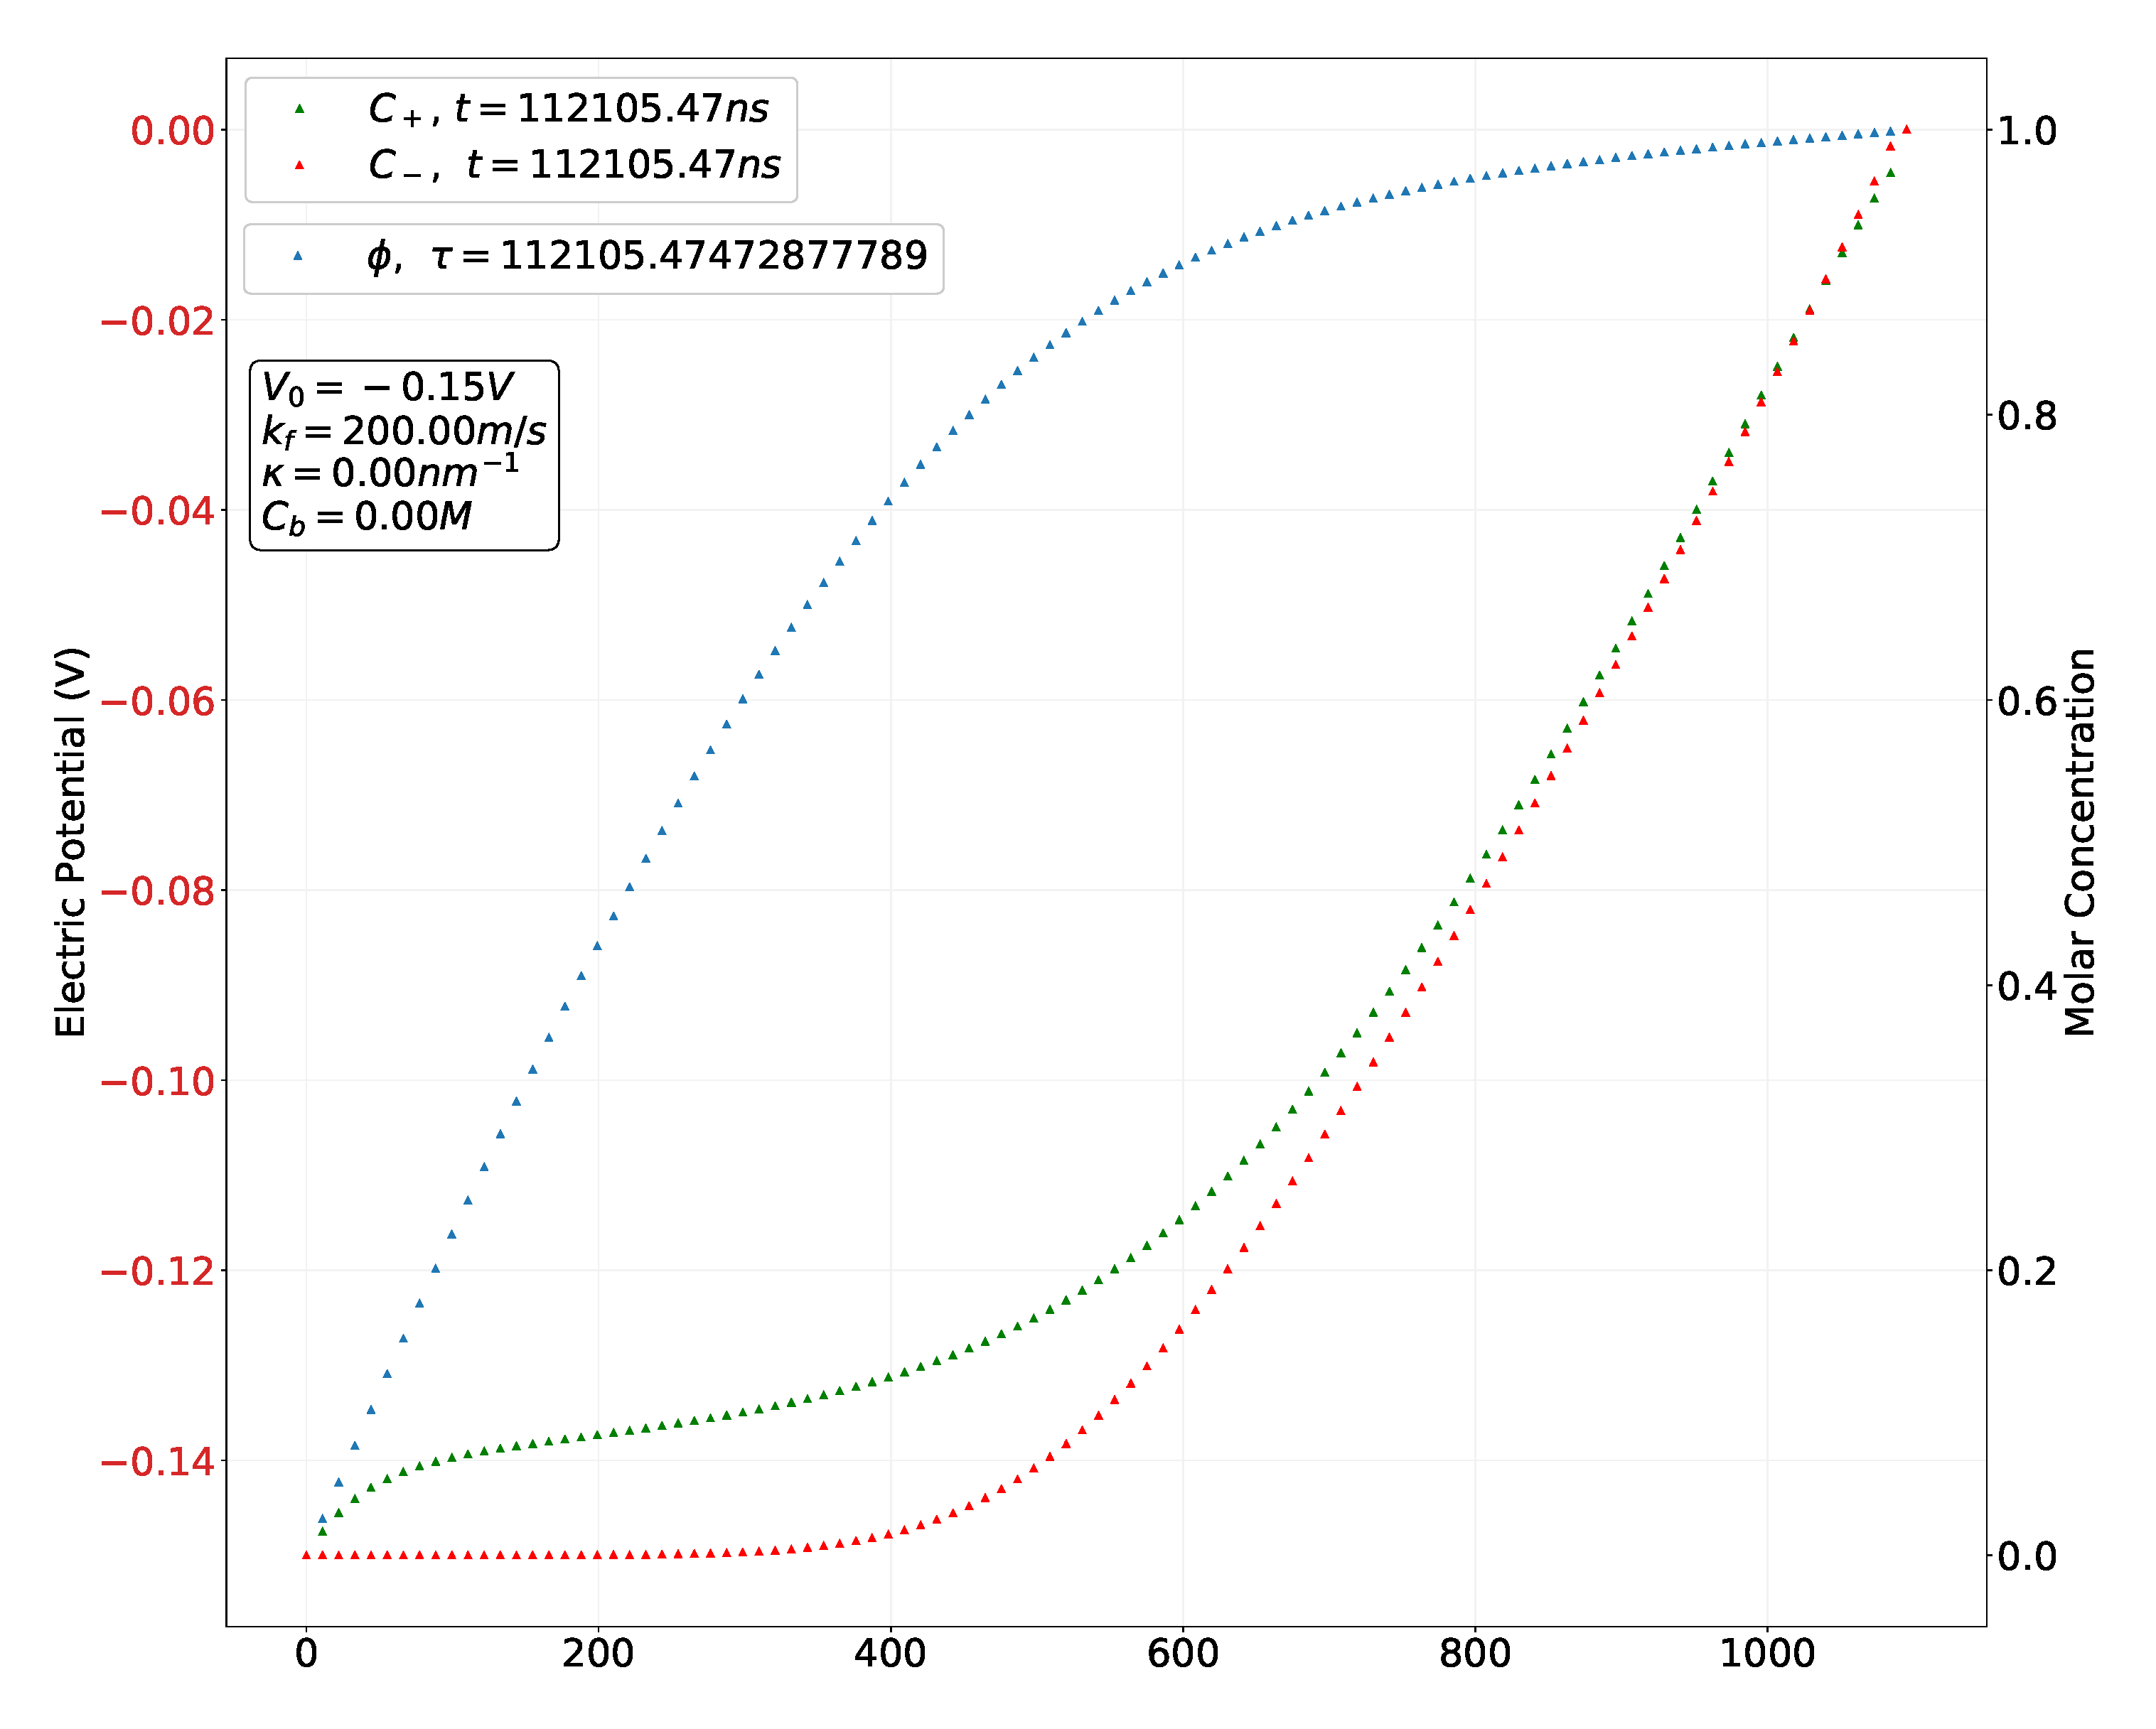
\includegraphics[width =\textwidth]{langmuir-diffusion-nernstphi1.eps}
\caption{}
\label{fig:time-evol2_2}
\end{subfigure}\\[1ex]
\begin{subfigure}{\linewidth}
\centering
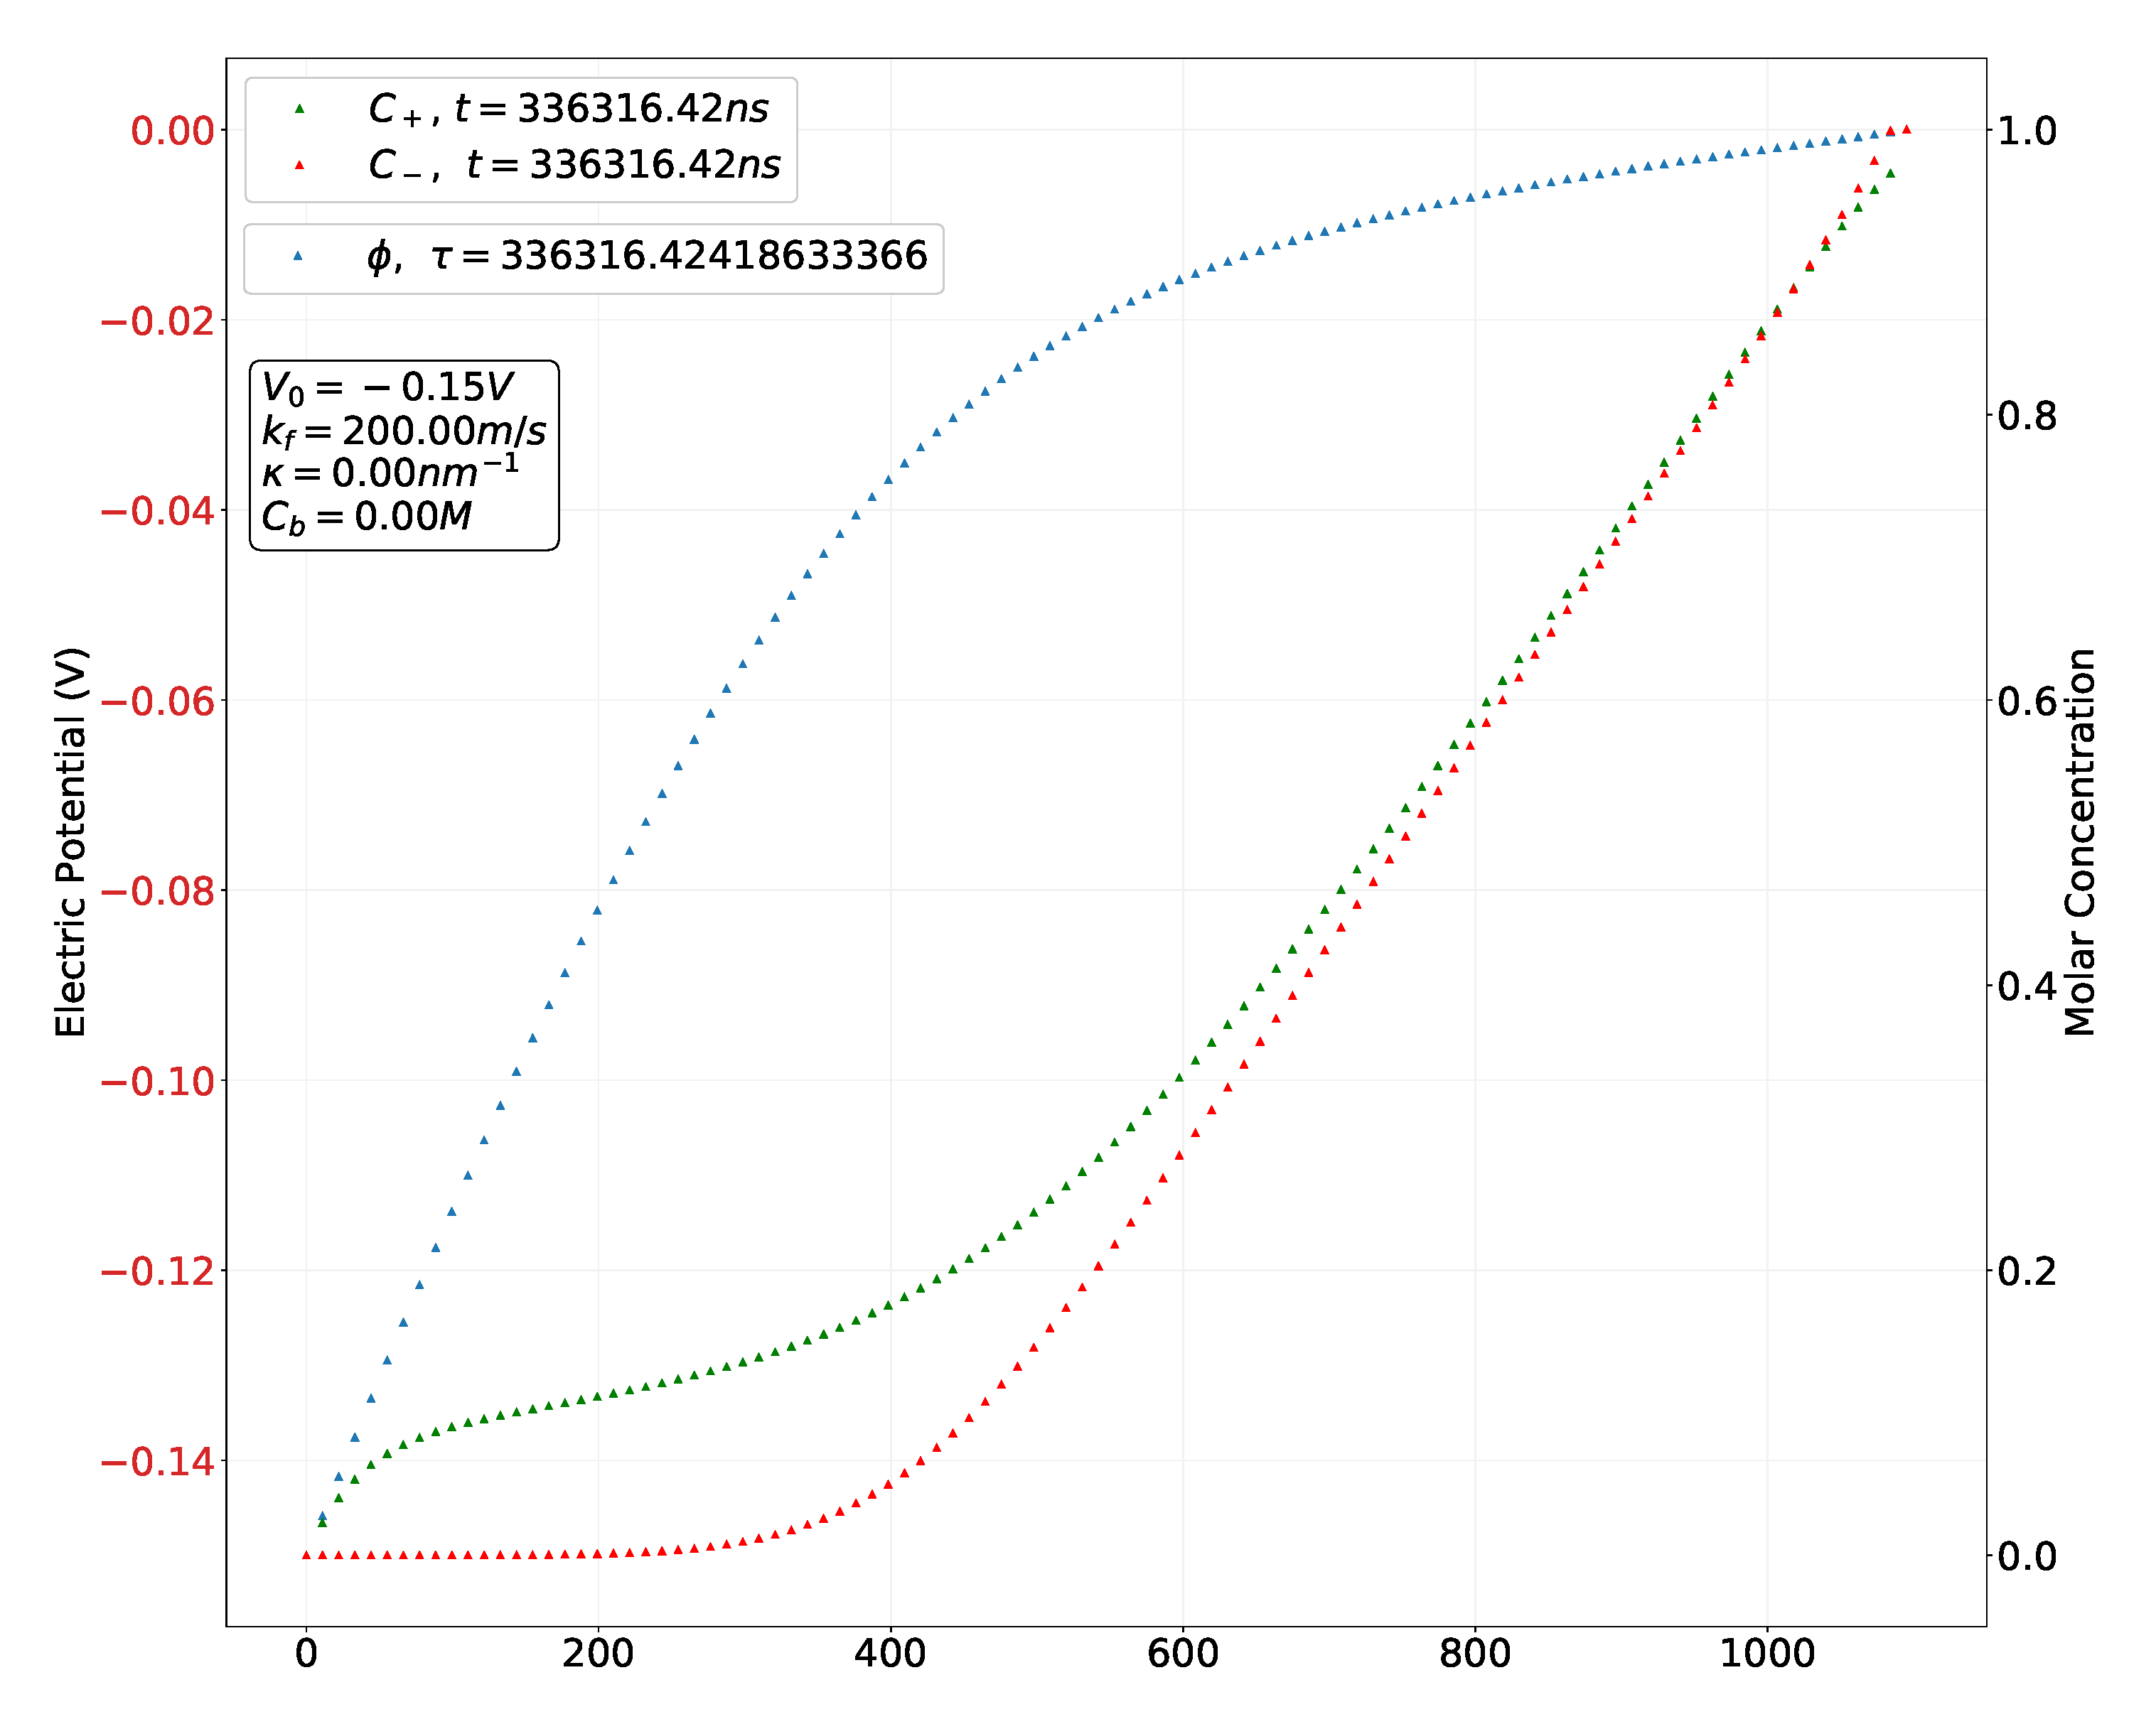
\includegraphics[width =0.5\textwidth]{langmuir-diffusion-nernstphi2.eps}
\caption{}
\label{fig:time-evol2_3}
\end{subfigure}
\caption{Electric potential in volts and molar concentration of $Cu^{+2}$ (green dots) and $SO_4^{-2}$ (blue dots) at (a) $t = 0.448 ns$, (b) $t = 2.24 ns$ and (c) $t = 4.44 ns$}
\label{fig:langmuir-diffusion-react}
\end{figure}


\newpage
\subsection{Electric field at the surface of the electrode}
\label{sec:analysis-efield}

A feature of interest is the electric field at the surface. As measurements by a solid state device would be done by implanting the device on the surface, we are interested in how would the electric field vary as the model's parameters fluctuate. Particularly, we are interested in how the electric field varies with voltage and with the bulk concentration.

\begin{figure}[htbp]
\centering
\textbf{Electric field at the surface.}\par\medskip
\begin{subfigure}{.5\linewidth}
\centering
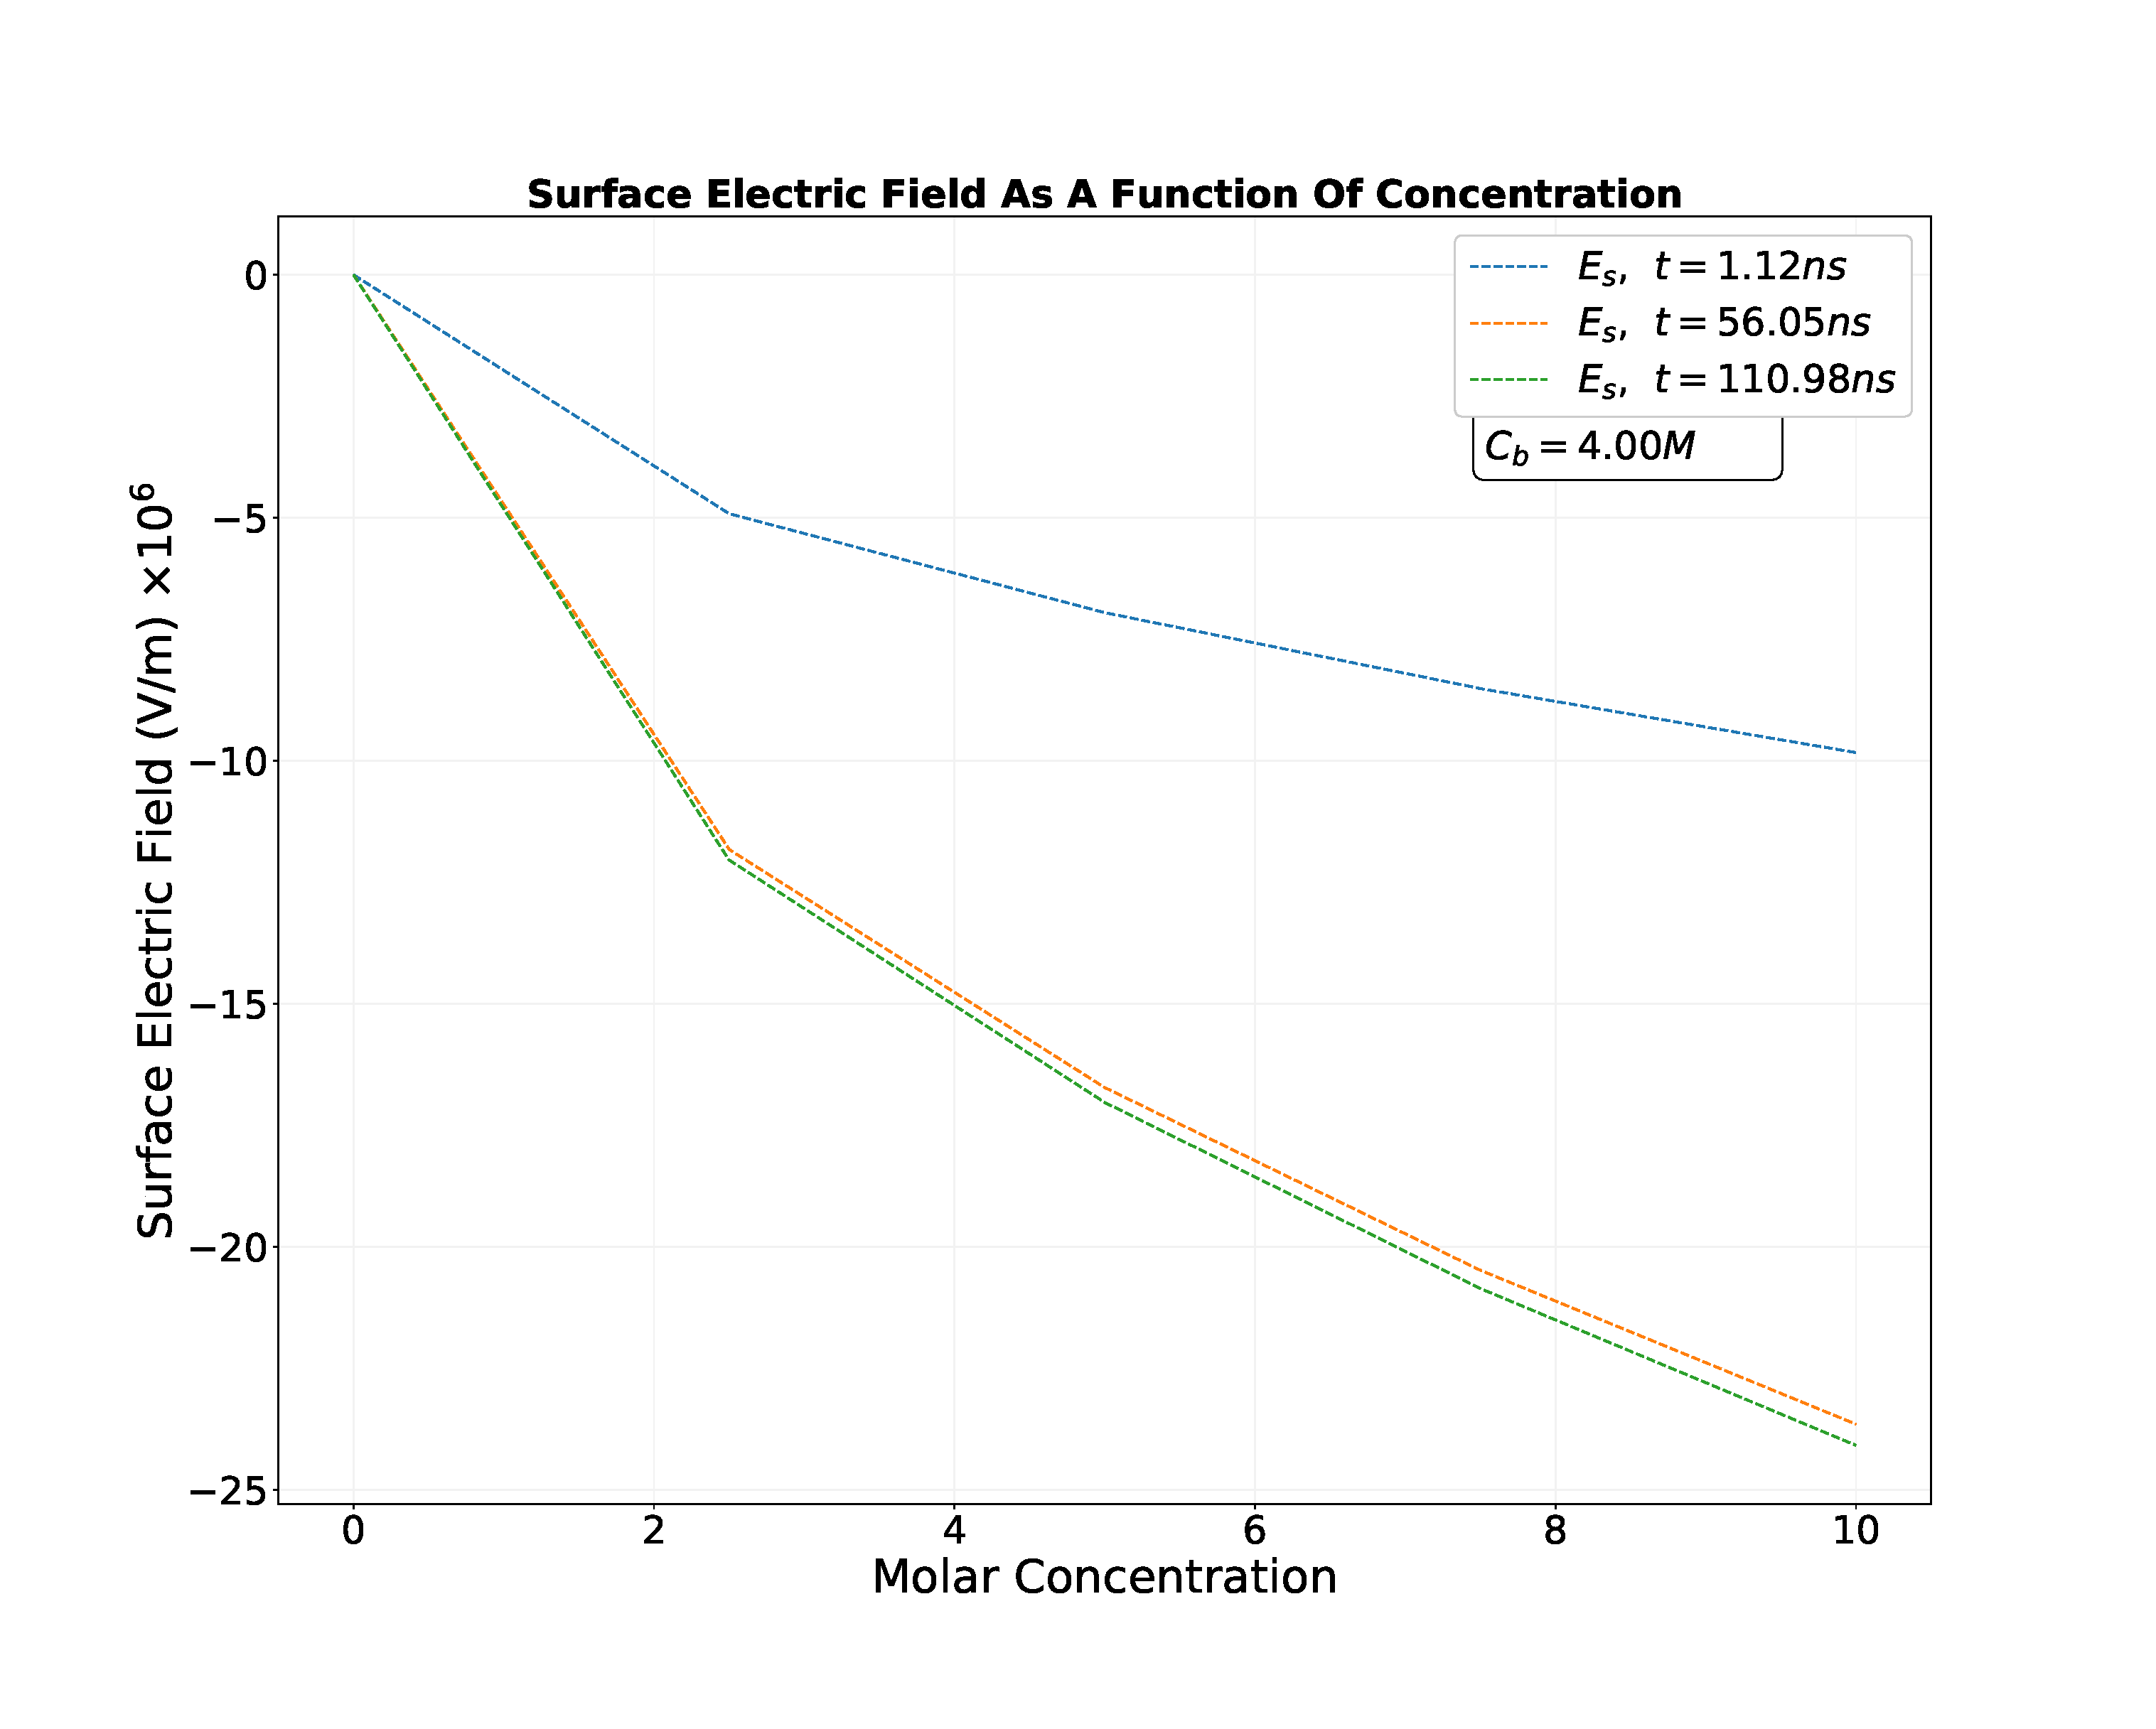
\includegraphics[width=\textwidth]{surfaceEfield_Cb.eps}
\caption{}
\label{fig:ef1}
\end{subfigure}%
\begin{subfigure}{.5\linewidth}
\centering
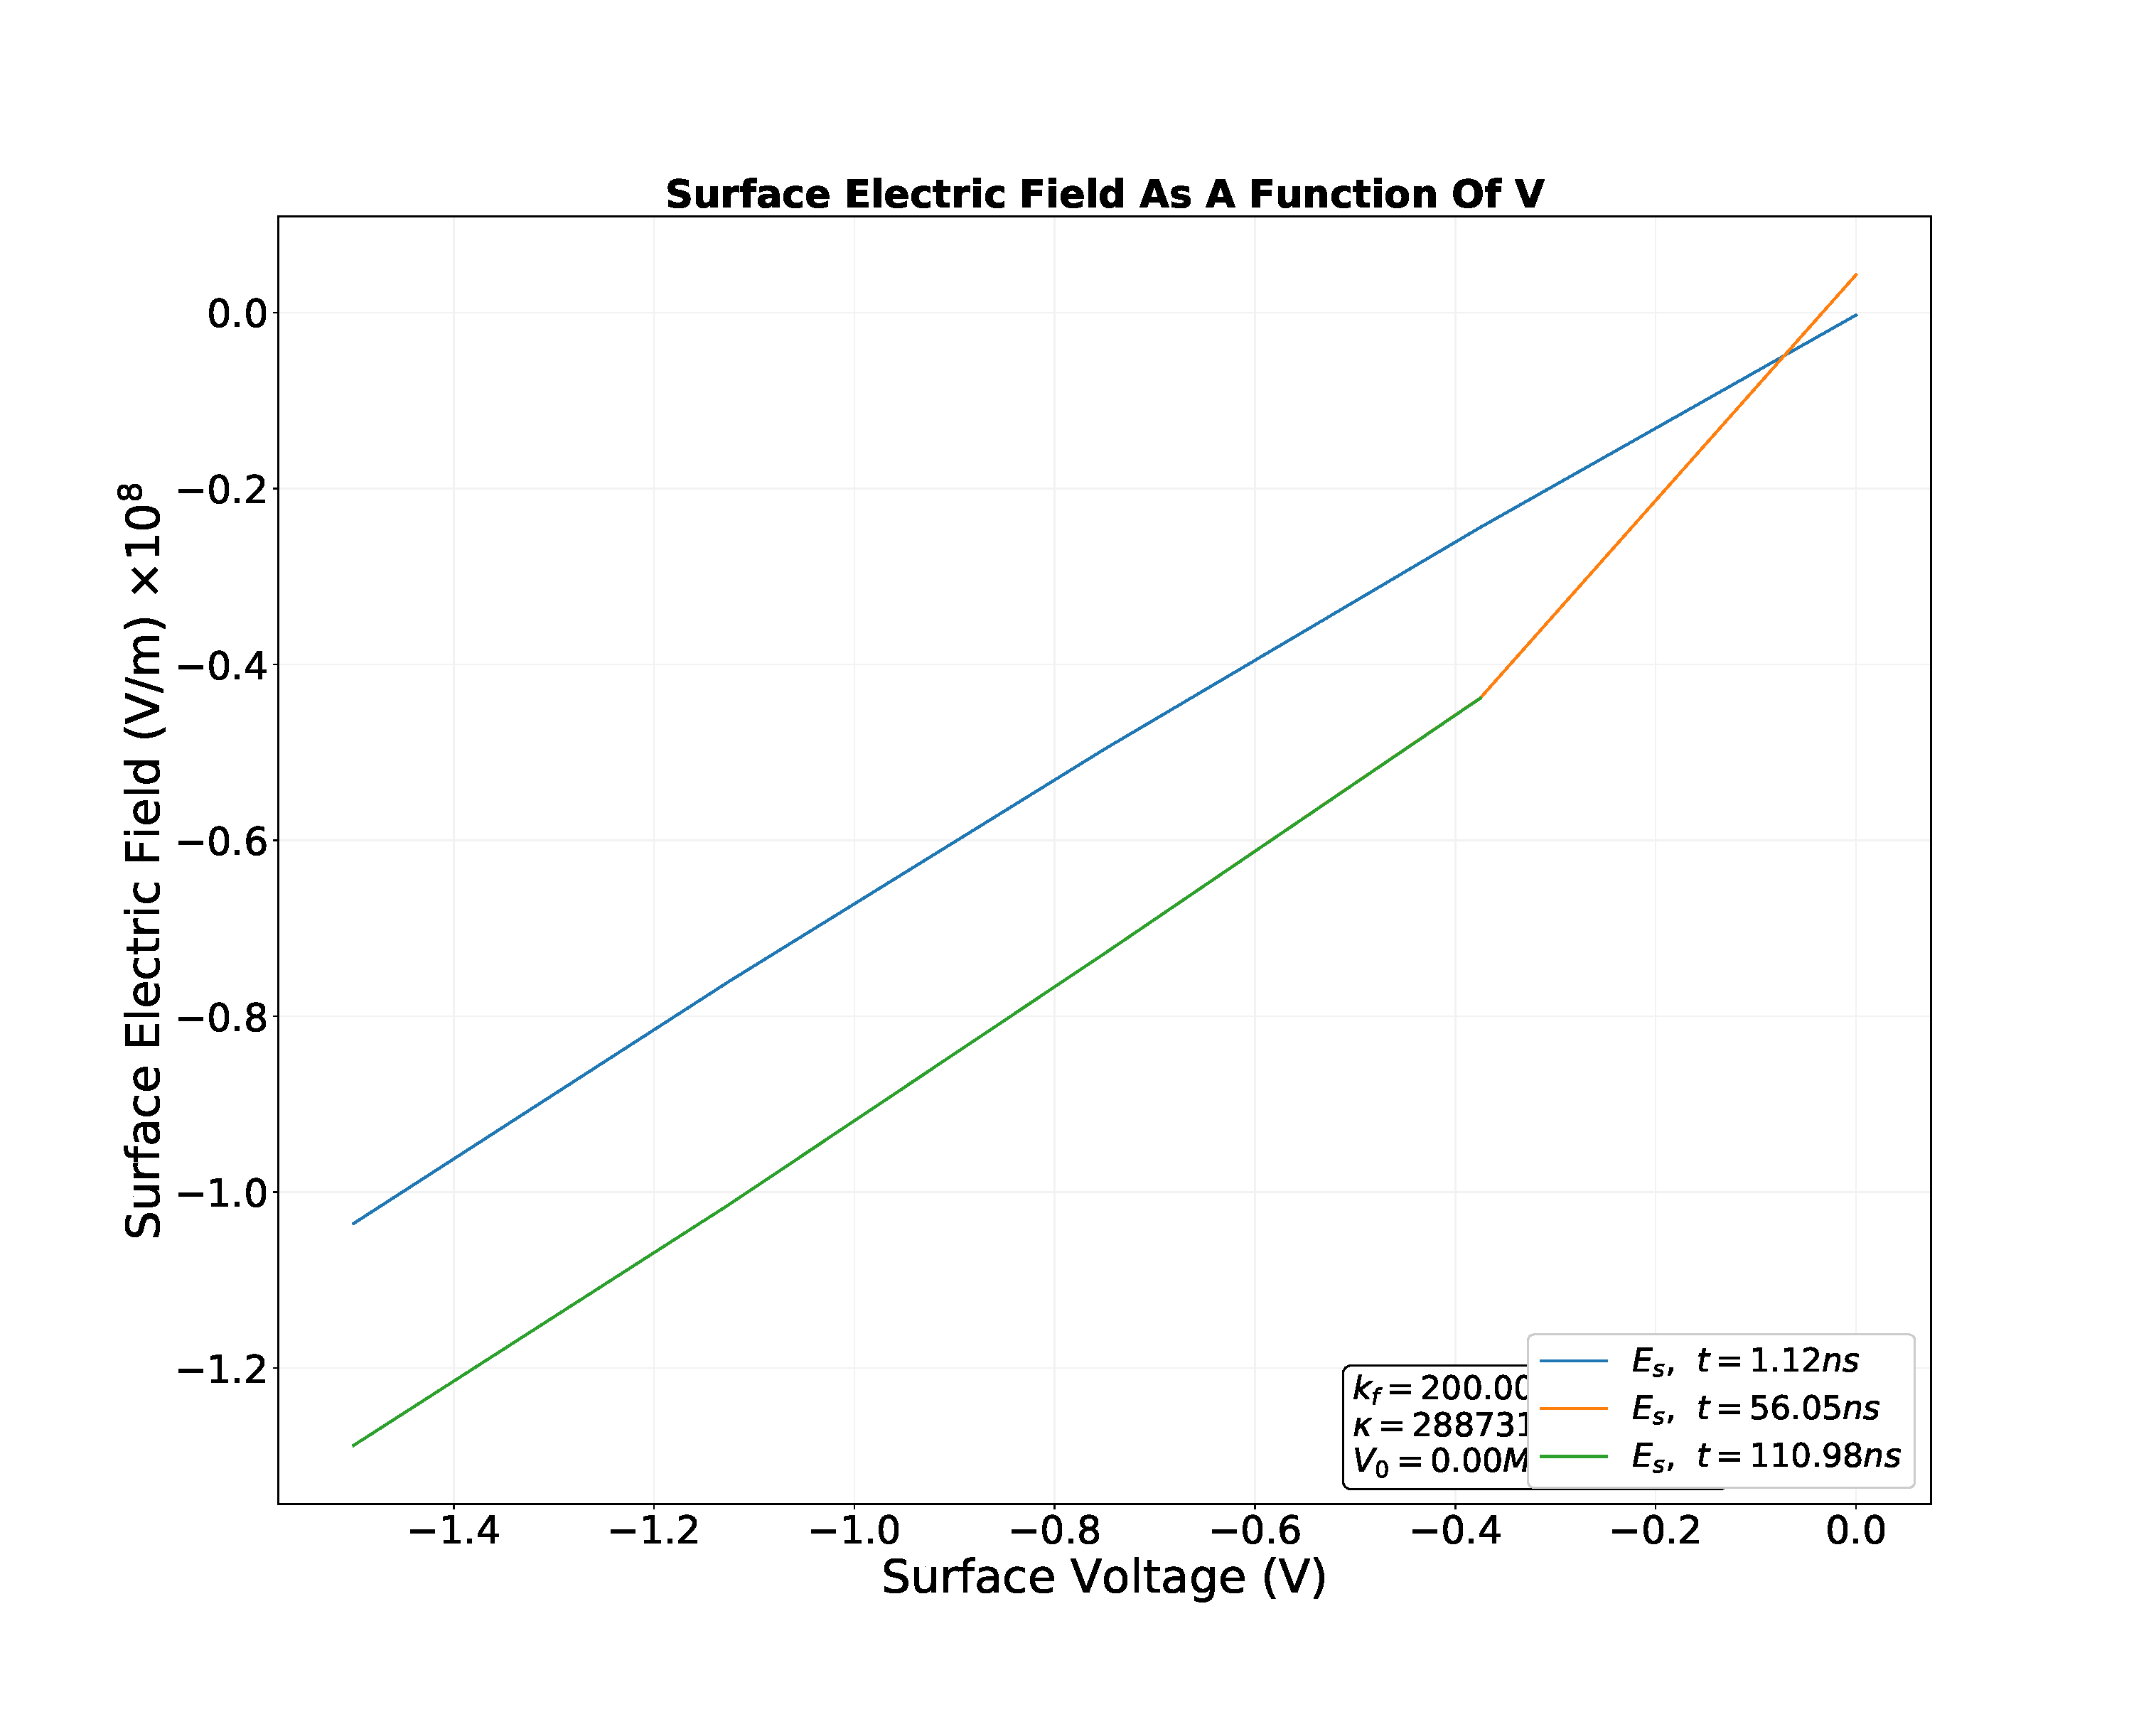
\includegraphics[width =\textwidth]{surfaceEfield_v.eps}
\caption{}
\label{fig:ef2}
\end{subfigure}\\[1ex]
\caption{(a) Electric field at the surface as a function of the molar concentration of the original salt. Dependence occurs through the model parameter $\kappa$ called the ionic force $\kappa$(b) Electric field at the surface $x=0$ of the electrode as a function of the voltage at the plate, which is a boundary condition to the Poisson equation \ref{eq:system}}
\end{figure}




\newpage
\subsection{Grounded electrode limit}

In the case of $V_0 = \Psi_0 = 0$ we get a purely diffusive process, as expected. 

\begin{figure}[htbp]
\centering
\includegraphics[width=\textwidth]{complete-no-electric-field.eps}
\caption{In the no-electrode limit we take $V_0=0$ in order to see the behavior diffusive-only limit. The electric field is zero throughout the system as an initial condition. The blue dots show the electric field due te the screening of the electrolyte in solution. }
\label{fig:nernts-no-field}
\end{figure}


\newpage
\subsection{Electric Field Fluctuation As A Function Of Time}


A quantity of great interest is the fluctuation of the electric field with respect to the steady state solution. Particularly, we are interested in studying such fluctuations at the interface with the electrode. Such fluctuations are defined as

\begin{align}
	\delta E(t) = E(x=0, t) - E_{SS}(x=0), 
\end{align}

where 

\begin{align}
	E_{SS}(x) = \lim_{t\rightarrow\infty} E(x,t).
\end{align}



\begin{figure}[htbp]
\centering
\includegraphics[width=\textwidth]{surfaceDeltaE.eps}
\caption{Electric field fluctuations at the electrode.}
\end{figure}

\newpage

The electric noise can be fitted with a polynomial curve in time which characterizes the noise. Fig. \ref{fig:efield-noise-fit} shows how the curves are fitted for different time concentration. Table \ref{table:fittin-params} shows the fitting parameters for each concentration value for the fitting curve

\begin{align}
	y(t) = a t + c
\end{align}

\begin{table}[htbp]
\centering
\begin{tabular}{lll}
$C_b$   & $a$           & $b$            \\\hline
$0.01M$ & $-0.00167455$ & $0.08372766$   \\
$0.3M$  & $-0.27515156$ & $13.7574389$   \\
$0.7M$  & $-0.98050493$ & $49.02044176$  \\
$1.2M$  & $-2.1993436$  & $109.92873245$
\end{tabular}
\caption{Fitting parameters for curves in Fig. \ref{fig:efield-noise-fit}}
\label{table:fittin-params}
\end{table}


\newpage
\begin{figure}[htbp]
\centering
\includegraphics[width=\textwidth]{surfaceDeltaE_fitting.eps}
\caption{Fitting the electric field fluctuations with a test function of the form $y(t) = a t + c$.}
\label{fig:efield-noise-fit}
\end{figure}




\newpage



